% TNSRE manuscript skeleton (draft). Every number is a macro from numbers.tex, generated from
% docs/figures/tnsre/figure_numbers.json by make_numbers.py; regenerate, never edit numbers by hand.
\documentclass[journal]{IEEEtran}
\usepackage{amsmath,amssymb}
\usepackage{graphicx}
\usepackage{xspace}
\xspaceaddexceptions{]}
\usepackage{booktabs}
\usepackage{xcolor}
\usepackage[hidelinks]{hyperref}
\graphicspath{{../figures/tnsre/}}
% generated by make_numbers.py from docs/figures/tnsre/figure_numbers.json; do not edit
\newcommand{\NumCommitPreregFreeze}{935c80a\xspace}
\newcommand{\NumCommitPreregAddendumAOne}{73626a0\xspace}
\newcommand{\NumCommitStageOne}{4e0d5fc\xspace}
\newcommand{\NumCommitStageTwo}{c8b1503\xspace}
\newcommand{\NumCommitUnderfitPlan}{8f89920\xspace}
\newcommand{\NumCommitTheoryThreeRule}{d54f0ef\xspace}
\newcommand{\NumCommitRobustnessPlan}{499972d\xspace}
\newcommand{\NumCommitIdentPlan}{8b4abe0\xspace}
\newcommand{\NumCommitIdentAThree}{cf0a65e\xspace}
\newcommand{\NumCommitIdentAFour}{a0013f4\xspace}
\newcommand{\NumCommitIdentAFourExt}{ce2d574\xspace}
\newcommand{\NumAlphaOne}{0.01\xspace}
\newcommand{\NumAlphaTwo}{0.04\xspace}
\newcommand{\NumTostBound}{0.10\xspace}
\newcommand{\NumNShuffles}{500\xspace}
\newcommand{\NumMinTrials}{40\xspace}
\newcommand{\NumTrfLagMax}{400\xspace}
\newcommand{\NumFsTrf}{64\xspace}
\newcommand{\NumFsRes}{256\xspace}
\newcommand{\NumNFc}{8\xspace}
\newcommand{\NumBandLo}{0.5\xspace}
\newcommand{\NumBandHi}{30\xspace}
\newcommand{\NumResSeed}{42\xspace}
\newcommand{\NumResRho}{0.9\xspace}
\newcommand{\NumResBeta}{0.05\xspace}
\newcommand{\NumResUnits}{256\xspace}
\newcommand{\NumNEeg}{32\xspace}
\newcommand{\NumCritOneAlpha}{0.01\xspace}
\newcommand{\NumCritTwoAlpha}{0.05\xspace}
\newcommand{\NumPowerPct}{80\xspace}
\newcommand{\NumCiPct}{95\xspace}
\newcommand{\NumTostCiPct}{90\xspace}
\newcommand{\NumLamSmall}{1\xspace}
\newcommand{\NumLamLarge}{10\xspace}
\newcommand{\NumLongTrf}{1000\xspace}
\newcommand{\NumRhoZero}{0\xspace}
\newcommand{\NumTempoRise}{4\xspace}
\newcommand{\NumSnrFactor}{8\xspace}
\newcommand{\NumTrialsFactor}{8\xspace}
\newcommand{\NumNestedDatasets}{10\xspace}
\newcommand{\NumLampairDatasets}{20\xspace}
\newcommand{\NumNTwo}{34\xspace}
\newcommand{\NumNOne}{8\xspace}
\newcommand{\NumNTrials}{3300\xspace}
\newcommand{\NumNTempi}{13\xspace}
\newcommand{\NumTempoMin}{1\xspace}
\newcommand{\NumTempoMax}{4\xspace}
\newcommand{\NumStageOneDelta}{0.091\xspace}
\newcommand{\NumStageOnePos}{6\xspace}
\newcommand{\NumStageOneP}{0.055\xspace}
\newcommand{\NumHTwoDelta}{0.228\xspace}
\newcommand{\NumHTwoLo}{0.121\xspace}
\newcommand{\NumHTwoHi}{0.277\xspace}
\newcommand{\NumHTwoPos}{31\xspace}
\newcommand{\NumHTwoP}{8.0\times10^{-9}\xspace}
\newcommand{\NumDriveDelta}{0.317\xspace}
\newcommand{\NumDriveLo}{0.228\xspace}
\newcommand{\NumDriveHi}{0.364\xspace}
\newcommand{\NumHOneLo}{$-$0.010\xspace}
\newcommand{\NumHOneHi}{+0.003\xspace}
\newcommand{\NumHThreeLo}{$-$0.007\xspace}
\newcommand{\NumHThreeHi}{+0.006\xspace}
\newcommand{\NumEnvLo}{0.162\xspace}
\newcommand{\NumEnvHi}{0.269\xspace}
\newcommand{\NumLinWorld}{0.039\xspace}
\newcommand{\NumLinWorldP}{7.3\times10^{-8}\xspace}
\newcommand{\NumPooledDelta}{0.245\xspace}
\newcommand{\NumPredDelta}{0.681\xspace}
\newcommand{\NumUDriveDelta}{0.315\xspace}
\newcommand{\NumSpectral}{0.156\xspace}
\newcommand{\NumSpectralLo}{0.113\xspace}
\newcommand{\NumSpectralHi}{0.231\xspace}
\newcommand{\NumPhase}{0.045\xspace}
\newcommand{\NumPhaseLo}{0.022\xspace}
\newcommand{\NumPhaseHi}{0.072\xspace}
\newcommand{\NumPhasePos}{26\xspace}
\newcommand{\NumPhaseP}{0.0003\xspace}
\newcommand{\NumRRs}{$-$0.0045\xspace}
\newcommand{\NumRRsLo}{$-$0.011\xspace}
\newcommand{\NumRRsHi}{+0.006\xspace}
\newcommand{\NumRRhoZero}{$-$0.0035\xspace}
\newcommand{\NumRRhoZeroLo}{$-$0.016\xspace}
\newcommand{\NumRRhoZeroHi}{+0.013\xspace}
\newcommand{\NumRhoCorr}{0.984\xspace}
\newcommand{\NumNRows}{11\xspace}
\newcommand{\NumNFlips}{0\xspace}
\newcommand{\NumTThreeDelta}{$-$0.010\xspace}
\newcommand{\NumTThreePos}{3\xspace}
\newcommand{\NumTThreeP}{1.00\xspace}
\newcommand{\NumTThreeLinDelta}{$-$0.004\xspace}
\newcommand{\NumTThreeAugVsLinP}{1.00\xspace}
\newcommand{\NumTThreeNegTempi}{13\xspace}
\newcommand{\NumRShort}{0.034\xspace}
\newcommand{\NumRLong}{0.028\xspace}
\newcommand{\NumRHopf}{0.020\xspace}
\newcommand{\NumRLin}{0.028\xspace}
\newcommand{\NumRRf}{0.006\xspace}
\newcommand{\NumRAug}{0.025\xspace}
\newcommand{\NumRAugLin}{0.031\xspace}
\newcommand{\NumGroupDelta}{$-$0.002\xspace}
\newcommand{\NumGroupPos}{8\xspace}
\newcommand{\NumGroupP}{1.00\xspace}
\newcommand{\NumSlopeLFull}{+0.484\xspace}
\newcommand{\NumSlopeLFullP}{0.0001\xspace}
\newcommand{\NumSlopeLFixed}{+0.015\xspace}
\newcommand{\NumSlopeLFixedP}{0.37\xspace}
\newcommand{\NumSlopeRFull}{+0.486\xspace}
\newcommand{\NumSlopeRFullP}{0.0006\xspace}
\newcommand{\NumSlopeRFixed}{+0.016\xspace}
\newcommand{\NumSlopeRFixedP}{0.45\xspace}
\newcommand{\NumOpR}{0.04\xspace}
\newcommand{\NumOpTrials}{40\xspace}
\newcommand{\NumOpTempi}{12\xspace}
\newcommand{\NumCalR}{0.040\xspace}
\newcommand{\NumNCells}{102\xspace}
\newcommand{\NumNDatasets}{20\xspace}
\newcommand{\NumNSimPart}{20\xspace}
\newcommand{\NumNKernels}{34\xspace}
\newcommand{\NumWA}{0.89\xspace}
\newcommand{\NumWAVar}{99\xspace}
\newcommand{\NumWB}{0.92\xspace}
\newcommand{\NumWNested}{0.96\xspace}
\newcommand{\NumWRefOne}{0.88\xspace}
\newcommand{\NumWRefTwo}{0.89\xspace}
\newcommand{\NumCMax}{0.10\xspace}
\newcommand{\NumFpMax}{0.00\xspace}
\newcommand{\NumFpHi}{0.17\xspace}
\newcommand{\NumOverlap}{0.53\xspace}
\newcommand{\NumRTwoShort}{62\xspace}
\newcommand{\NumRTwoShortMin}{29\xspace}
\newcommand{\NumRTwoShortMax}{85\xspace}
\newcommand{\NumRTwoLong}{82\xspace}
\newcommand{\NumCritOneA}{0.58\xspace}
\newcommand{\NumCritOneB}{0.58\xspace}
\newcommand{\NumCritOneC}{0.47\xspace}
\newcommand{\NumCritOneNestedA}{0.59\xspace}
\newcommand{\NumCritOneNestedALo}{0.5\xspace}
\newcommand{\NumCritOneNestedAHi}{0.6\xspace}
\newcommand{\NumTierB}{0.59\xspace}
\newcommand{\NumTierBPct}{59\xspace}
\newcommand{\NumEvokedOnly}{$-$0.0067\xspace}
\newcommand{\NumHopfSpecA}{5\xspace}
\newcommand{\NumHopfSpecC}{18\xspace}
\newcommand{\NumRealDelta}{$-$0.010\xspace}
\newcommand{\NumRealPos}{3\xspace}
\newcommand{\NumRealP}{1.00\xspace}
\newcommand{\NumCritTwoACommitted}{20\xspace}
\newcommand{\NumCritTwoAOne}{0\xspace}
\newcommand{\NumCritTwoATen}{18\xspace}
\newcommand{\NumCritTwoANested}{10\xspace}
\newcommand{\NumCritTwoCCommitted}{1\xspace}
\newcommand{\NumCritTwoCOne}{1\xspace}
\newcommand{\NumCritTwoCTen}{20\xspace}
\newcommand{\NumCritTwoCNested}{0\xspace}
\newcommand{\NumCritTwoACommittedN}{20\xspace}
\newcommand{\NumCritTwoANestedN}{10\xspace}
\newcommand{\NumCritTwoCCommittedN}{20\xspace}
\newcommand{\NumCritTwoCNestedN}{10\xspace}
\newcommand{\NumCritOneNestedC}{0.5\xspace}
\newcommand{\NumCritOneNestedCText}{at or below 0.5\xspace}

% claim labels
\newcommand{\Conf}{\textsc{[confirmatory]}\xspace}
\newcommand{\Expl}{\textsc{[exploratory]}\xspace}
\newcommand{\Simul}{\textsc{[simulated]}\xspace}
\newcommand{\CITEQ}[1]{\textcolor{red}{[CITE?: #1]}}

\begin{document}
\title{What a Linear Encoding Model Leaves at the Beat: A Pre-Registered Test of Residual Beat-Locking, a Spiking-Reservoir Readout, and the Identifiability Limits of Oscillator-versus-Evoked Comparisons in Single-Listen EEG}
\author{[Authors to be added]% do not invent names or affiliations
\thanks{Manuscript draft. Pre-registration frozen at commit \NumCommitPreregFreeze of the project repository.}}
\markboth{IEEE Transactions on Neural Systems and Rehabilitation Engineering (draft)}{}
\maketitle

\begin{abstract}
Whether beat-locked EEG reflects entrained oscillators or summed evoked responses is often argued from frequency-tagging magnitudes, which cannot separate the two. We asked a narrower, testable question: does fronto-central EEG keep beat-locked power after a cross-validated linear encoding model of the music, a temporal response function (TRF), is removed? In a pre-registered two-stage test on \NumNTwo participants listening to music at \NumNTempi tempi (Weineck et al.\ 2022 data), the residual kept beat-locked power (\Conf; median standardized effect \NumHTwoDelta, \NumHTwoPos/\NumNTwo positive). A fixed spiking reservoir (ARSPI-Net, \NumResUnits leaky integrate-and-fire units) read out linearly was equivalent to the linear statistic (H1, H3; \Conf). A copy with shuffled reservoir weights matched it (\Expl). Exploratory checks showed the residual is not explained by underfitting (linear-world residual \NumLinWorld) and splits into a spectral part (\NumSpectral) and a smaller phase-dependent part (\NumPhase). Oscillator-bank encoding models did not beat the TRF at held-out tempi (\Expl). A simulation map of that comparison (\Simul) showed the committed rule has no false positives but reaches \NumPowerPct\% power only for an oscillator supplying a share of about \NumWA of the stimulus-locked amplitude, and that its Hopf-versus-linear-bank criterion has no regularization-stable answer. Under the real pipeline's regularization procedure, the real data bound oscillatory structure beyond the TRF below about \NumTierBPct\% of the stimulus-locked amplitude (\Expl). We provide a calibrated identifiability procedure for encoding-model tests of entrainment.
\end{abstract}

\begin{IEEEkeywords}
EEG, neural entrainment, temporal response function, reservoir computing, spiking neural network, pre-registration, identifiability.
\end{IEEEkeywords}

\section{Introduction}
Rhythmic music drives EEG activity at the beat frequency, and whether this reflects endogenous oscillators entrained by the stimulus or a superposition of transient evoked responses is a long-running question \cite{doelling2021neural,breska2017delta,vanbree2021sustained}. Frequency-tagging magnitudes alone do not distinguish the two accounts \cite{nozaradan2011tagging,henry2017what,zhou2016interpretations,novembre2018tagging,rajendran2019frequency,doelling2019oscillator,damsma2025tempo}, and encoding models (temporal response functions, TRFs) describe stimulus-locked responses without settling the mechanism~\cite{crosse2016mtrf}.

We replace the mechanism question with three that the data can answer: (i) after a cross-validated linear encoding model of four music features is subtracted, does beat-locked power remain (H2)? (ii) does a fixed spiking reservoir add detection power over a linear statistic (H1, H3)? (iii) at held-out tempi, does an oscillator encoding model predict the EEG better than the TRF, and how large an oscillator contribution could that comparison detect at single-listen signal-to-noise ratio? The first two were pre-registered (\Conf); the third, and every check around the first two, is labelled \Expl or \Simul. The reservoir is the canonical ARSPI-Net leaky integrate-and-fire (LIF) reservoir \cite{lane2024towards}, used here as a characterized instrument rather than a classifier \cite{verstraeten2007experimental,soures2019spiking}.

Contributions: (1) a pre-registered, calibrated residual beat-tagging test with its null validated and rejected nulls recorded; (2) an equivalence result for a fixed spiking reservoir against its linear readout; (3) an identifiability map of the oscillator-versus-evoked held-out-tempo comparison, showing where it can and cannot decide and how much of its answer depends on the regularization of the comparison models.

\section{Methods}
\subsection{Data}
We used the openly available EEG of Weineck, Wen and Henry \cite{weineck2022neural}, deposited on OSF (doi:10.17605/OSF.IO/Y5XHS) under a CC~BY~4.0 licence: \NumNTwo participants, \NumNEeg channels, music at \NumNTempi tempi from \NumTempoMin to \NumTempoMax\,Hz. Stimulus features (spectral flux, beat onsets, envelope and its derivative) were taken from the authors' source data and matched to trials by duration one-to-one; trials with ambiguous matches were dropped. EEG was band-passed \NumBandLo--\NumBandHi\,Hz, average-referenced and resampled to \NumFsTrf\,Hz for the TRF and \NumFsRes\,Hz for the reservoir; the target was the mean of \NumNFc fronto-central channels. Stage 2 used \NumNTrials one-to-one trials; every participant met the pre-registered minimum of \NumMinTrials trials.

\subsection{Pre-registration and timeline}
The pre-registration (two-stage design, hypotheses, statistic, null, equivalence bounds) was frozen at commit \NumCommitPreregFreeze before any group test; addendum A1 (commit \NumCommitPreregAddendumAOne) recorded before the stage-1 group test that stage 1 had \NumNOne participants. Stage 1 tested H2 at $\alpha=\NumAlphaOne$; stage 2 (all \NumNTwo participants, downloaded unconditionally) at $\alpha=\NumAlphaTwo$. Stage-1 and stage-2 results were committed at \NumCommitStageOne and \NumCommitStageTwo. Every exploratory analysis had its plan and decision rule committed before it ran: underfitting check \NumCommitUnderfitPlan, oscillator decision rule \NumCommitTheoryThreeRule, robustness grid \NumCommitRobustnessPlan, identifiability plan \NumCommitIdentPlan, addenda A3 \NumCommitIdentAThree and A4 \NumCommitIdentAFour (extension \NumCommitIdentAFourExt).

\subsection{Residual beat-tagging}
Per participant, a ridge TRF (lags 0--\NumTrfLagMax\,ms, four features, regularization chosen by nested leave-one-trial-out cross-validation) predicted each held-out trial; the residual is the EEG minus that prediction. Beat-locking was scored with one statistic for every signal: Welch power at the trial's own tempo and its octave, relative to a local baseline, compared with the same score at the other grid tempi. The per-trial standardized effect $\delta$ is the mean over trials of own-tempo minus mean other-tempo score, divided by its standard deviation across trials. The null shuffles stimulus labels across trials (\NumNShuffles shuffles); nulls that fail on a periodic grid (circular shift, phase randomization) or inflated false positives in calibration were rejected and are recorded in the pre-registration. H2: residual $\delta>0$ (one-sided Wilcoxon signed-rank over participants). H1/H3: reservoir minus linear statistic on the drive and on the residual, equivalent within $\pm\NumTostBound\,\delta$ by two one-sided tests~\cite{lakens2017equivalence}.

\subsection{ARSPI-Net reservoir}
The canonical reservoir has \NumResUnits LIF units, leak $\beta=\NumResBeta$, spectral radius $\rho=\NumResRho$, seed \NumResSeed; it is driven by the (residual or raw) fronto-central signal at \NumFsRes\,Hz and read out linearly as the first principal component across units (R). A copy with shuffled recurrent weights rescaled to the same spectral radius (Rs) tests whether the recurrent structure matters \cite{verstraeten2007experimental,soures2019spiking,lane2024towards}.

\subsection{Exploratory checks of H2}
(i) Underfitting: a pooled leave-one-participant-out TRF; the tagging of the TRF prediction itself; and a linear world (fitted kernels convolved with the real features plus noise matched to the observed held-out $r$) through the identical pipeline. (ii) IAAFT surrogates of the residual \cite{theiler1992testing,schreiber1996improved}, splitting $\delta$ into a part the surrogates keep (spectral) and a part they destroy (phase-dependent). (iii) A robustness grid of \NumNRows rows (seeds, $\rho$, $\beta$, TRF variants, IAAFT). (iv) The \NumNTempi-tempo curve rescored on a fixed number of beat cycles per tempo.

\subsection{Oscillator encoding models (Theory 3)}
Banks of driven Hopf (Stuart--Landau) oscillators, resonate-and-fire units and linear damped oscillators \cite{large2010canonical,large2015neural,izhikevich2001resonateandfire} were driven by the beat-related features; their lagged outputs, alone or added to the TRF, were fitted by ridge regression and evaluated at held-out tempi (leave-one-tempo-out, configuration and regularization chosen in an inner loop). The committed rule: the Hopf-augmented model beats the best TRF (median $\Delta r>0$, one-sided Wilcoxon $p<\NumCritOneAlpha$; criterion 1) and beats the linear-bank-augmented model ($p<\NumCritTwoAlpha$; criterion 2).

\subsection{Identifiability simulation}
Simulated participants used real fitted kernels (\NumNKernels participants) and real stimulus features: the signal was $s=(1-w)P_e/\mathrm{sd}_e+wP_o/\mathrm{sd}_o$, with $P_e$ the evoked (TRF) prediction, $P_o$ the Hopf-bank prediction and $w$ the oscillator's amplitude share, plus noise with the pooled residual spectrum scaled to a target held-out $r$ (calibrated: \NumCalR at a target of \NumOpR). Each cell ran \NumNDatasets datasets of \NumNSimPart participants through the identical leave-one-tempo-out comparison and the committed rule, computed from per-trial sufficient statistics with the modal regularization of the real data. World A is the committed grid (held-out $r$, trials per tempo, training tempi, $w$). Addendum A3 added World B (signal variance held constant across $w$), World C ($P_o$ replaced by its residual after projection onto the TRF design, i.e.\ only TRF-inexpressible oscillator structure) and a nested-regularization check; addendum A4 added nested-regularization cells for criterion 1 and a lambda-pair sensitivity analysis of criterion 2. Rates carry \NumCiPct\% Clopper--Pearson intervals~\cite{clopper1934use}; W80 is the interpolated $w$ at \NumPowerPct\% detection.

\section{Results}
\subsection{H2: beat-locked power beyond the linear encoding model}
Stage 1 (\NumNOne participants) did not reach its threshold ($p=\NumStageOneP$ against $\alpha=\NumAlphaOne$; median $\delta$ \NumStageOneDelta). At stage 2 (\Conf) the residual kept beat-locked power: median $\delta=\NumHTwoDelta$ [\NumHTwoLo, \NumHTwoHi], \NumHTwoPos/\NumNTwo positive, $p=\NumHTwoP$ (Fig.~\ref{fig:conf}a; drive \NumDriveDelta [\NumDriveLo, \NumDriveHi]). This is a statement about this linear encoding model, not about oscillators. \Expl The linear world left \NumLinWorld against the real \NumHTwoDelta ($p=\NumLinWorldP$), and a pooled TRF left \NumPooledDelta, so underfitting does not account for it (Fig.~\ref{fig:under}a). IAAFT surrogates retained \NumSpectral [\NumSpectralLo, \NumSpectralHi] (spectral) and removed \NumPhase [\NumPhaseLo, \NumPhaseHi] (phase-dependent; \NumPhasePos/\NumNTwo positive, $p=\NumPhaseP$; Fig.~\ref{fig:under}b): the residual beat-locking is nonlinear relative to the TRF and predominantly spectral, with a smaller reliable phase-coherent part. No robustness row flipped H2 (\NumNFlips of \NumNRows; Fig.~\ref{fig:rob}).

\subsection{The reservoir is equivalent to its linear readout}
\Conf On the drive and on the residual, the reservoir statistic was equivalent to the linear statistic (\NumTostCiPct\% intervals \NumHOneLo to \NumHOneHi and \NumHThreeLo to \NumHThreeHi, inside $\pm\NumTostBound$; Fig.~\ref{fig:conf}b). It exceeded envelope and squared statistics (\NumEnvLo to \NumEnvHi) only because those were null on the residual. \Expl Shuffling the recurrent weights changed nothing (R$-$Rs \NumRRs [\NumRRsLo, \NumRRsHi]), nor did removing recurrence (R at $\rho=\NumResRho$ minus R at $\rho=\NumRhoZero$: \NumRRhoZero [\NumRRhoZeroLo, \NumRRhoZeroHi]; per-participant correlation \NumRhoCorr; Fig.~\ref{fig:res}). The H2 statistic itself never passes through the reservoir, so its robustness rows over seed, $\rho$ and $\beta$ are identical by construction.

\subsection{Oscillator encoding models at held-out tempi}
\Expl Under the rule fixed in advance, the oscillator account was not supported: Hopf-augmented minus best TRF median $\Delta r$ \NumTThreeDelta, \NumTThreePos/\NumNTwo positive ($p=\NumTThreeP$), negative at \NumTThreeNegTempi of \NumNTempi held-out tempi, with no preferred rate (Fig.~\ref{fig:t3}a,b); pooled across participants \NumGroupDelta (\NumGroupPos/\NumNTwo positive). The apparent rise of tagging toward \NumTempoRise\,Hz did not survive a fixed number of beat cycles per tempo (participant slopes \NumSlopeLFull\,z/Hz, $p=\NumSlopeLFullP$, full duration; \NumSlopeLFixed, $p=\NumSlopeLFixedP$, fixed cycles; Fig.~\ref{fig:t3}c).

\subsection{What the comparison can decide: identifiability}
\Simul At the operating point of these data (held-out $r$ \NumOpR, \NumOpTrials trials per tempo, \NumOpTempi training tempi) the committed rule had no false positives (maximum rate \NumFpMax, upper \NumCiPct\% bound \NumFpHi with \NumNDatasets datasets) and reached \NumPowerPct\% detection only at an oscillator amplitude share of \NumWA (\NumWAVar\% of the variance), unchanged by a \NumSnrFactor-fold change in held-out $r$ or a \NumTrialsFactor-fold change in trial count, by power matching (World B, \NumWB) and in refined cells (\NumWRefOne, \NumWRefTwo); World C, the TRF-inexpressible oscillator, was never detected (maximum rate \NumCMax) (Fig.~\ref{fig:ident}). The two generating predictions overlap (median $r$ \NumOverlap), and the TRF design expresses a median \NumRTwoShort\% of the oscillator prediction's variance (range \NumRTwoShortMin--\NumRTwoShortMax\%; \NumRTwoLong\% for a 0--\NumLongTrf\,ms TRF).

\Expl (outside the committed rule) The limit sits in criterion 2. Criterion 1 alone reached \NumPowerPct\% at $w=\NumCritOneA$ (World A), \NumCritOneB (B) and \NumCritOneC (C) with fixed regularization, and at \NumCritOneNestedA (World A, bracket \NumCritOneNestedALo--\NumCritOneNestedAHi) and \NumCritOneNestedCText (World C) under the real pipeline's nested regularization. Criterion 2 has no regularization-stable answer: at $w=1$ it passed in World A in \NumCritTwoACommitted/\NumCritTwoACommittedN datasets with the committed pair, \NumCritTwoAOne/\NumLampairDatasets with both models at $\lambda=\NumLamSmall$, \NumCritTwoATen/\NumLampairDatasets at $\lambda=\NumLamLarge$ and \NumCritTwoANested/\NumCritTwoANestedN under nested selection; in World C \NumCritTwoCCommitted/\NumCritTwoCCommittedN, \NumCritTwoCOne/\NumLampairDatasets, \NumCritTwoCTen/\NumLampairDatasets and \NumCritTwoCNested/\NumCritTwoCNestedN. With each model at its own inner-loop regularization, the rule detected World A at W80 \NumWNested and never detected World C.

\Expl Placement of the real data: criterion 1 itself failed (median $\Delta r$ \NumRealDelta, \NumRealPos/\NumNTwo positive, $p=\NumRealP$), below the simulated evoked-only world (\NumEvokedOnly). Taking the largest criterion-1 W80 among the worlds as the conservative bound, the real data exclude, at about \NumPowerPct\% power, oscillatory structure beyond the TRF supplying more than about \NumTierBPct\% of the stimulus-locked amplitude.

\section{Discussion}
Residual beat-locked power beyond a four-feature linear encoding model is real in these data and is not an underfitting artifact; most of it is spectral, so a linear model with different features or a nonlinear stimulus-response map could absorb it \cite{declercq2022beyond,wilroth2024nonlinearity}. Neither the spiking reservoir nor its recurrence added detection power, which makes the reservoir a calibrated, scaled copy of its input in the beat band rather than a detector of structure the linear statistic misses; this is a measured, negative result about the instrument. The oscillator-versus-evoked comparison at held-out tempi did not favor oscillators, but the identifiability map limits what that null means: the committed rule cannot see an oscillator supplying half the amplitude, and its Hopf-versus-linear criterion changes verdict with the regularization of the comparison model. A methods lesson follows: encoding-model comparisons of mechanism need identifiability maps at the data's own SNR, and comparison-model regularization must be reported as part of the result. Designs that perturb rhythm (missing beats, tempo changes, offset persistence with ringing controls) are where the distinction can live \cite{tal2017neural,vanbree2021sustained,pesnotlerousseau2021frequency}.

\section{Limitations}
Single dataset with one listening paradigm; generalization to naturalistic single listens (NMED-T~\cite{losorelli2017ismir}) is pending. The TRF uses four features and 0--\NumTrfLagMax\,ms lags; other feature sets may absorb part of the residual. Stage 1 alone was inconclusive and H2 rests on stage 2. The identifiability simulation fixes the oscillator configuration, uses Gaussian noise with a smooth spectrum, \NumNSimPart participants per dataset (the real group had \NumNTwo) and \NumNDatasets datasets per cell; nested-regularization cells had \NumNestedDatasets. Exploratory analyses are post hoc relative to the confirmatory tests, though each plan was committed before it ran.

\section*{Data and Code Availability}
EEG: Weineck et al.\ \cite{weineck2022neural}, CC BY 4.0, not redistributed. Code, aggregate results, pre-registration and all plans: project repository [URL to be added]; every number in this manuscript is generated from the results files by \texttt{make\_numbers.py}.

\begin{figure*}[!t]\centering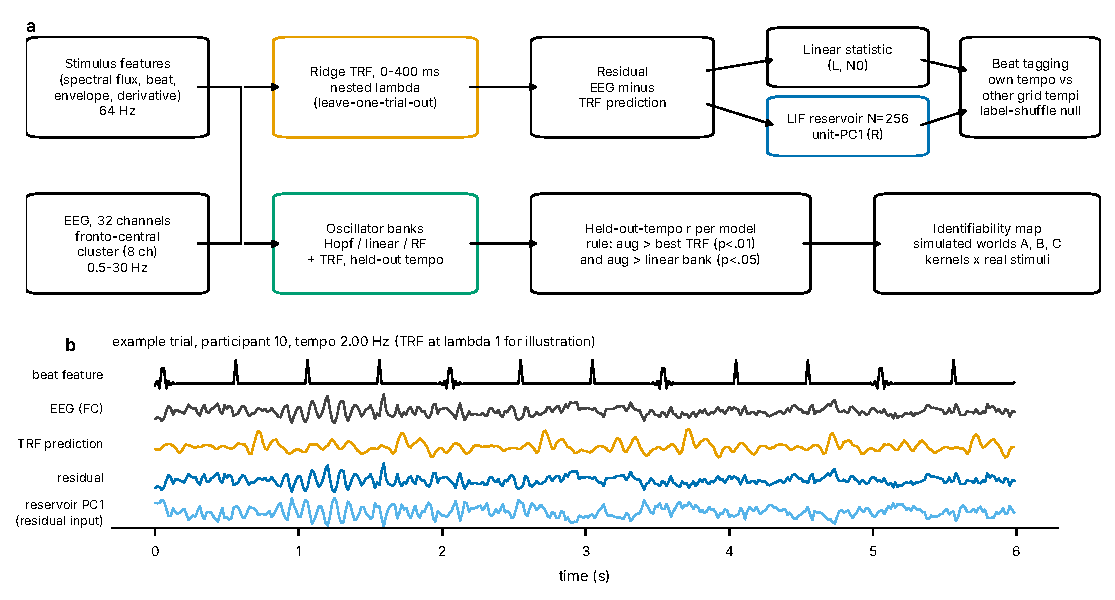
\includegraphics[width=\textwidth]{fig1_pipeline.pdf}\caption{Pipeline and example trial (see docs/FIGURES.md).}\label{fig:pipe}\end{figure*}
\begin{figure*}[!t]\centering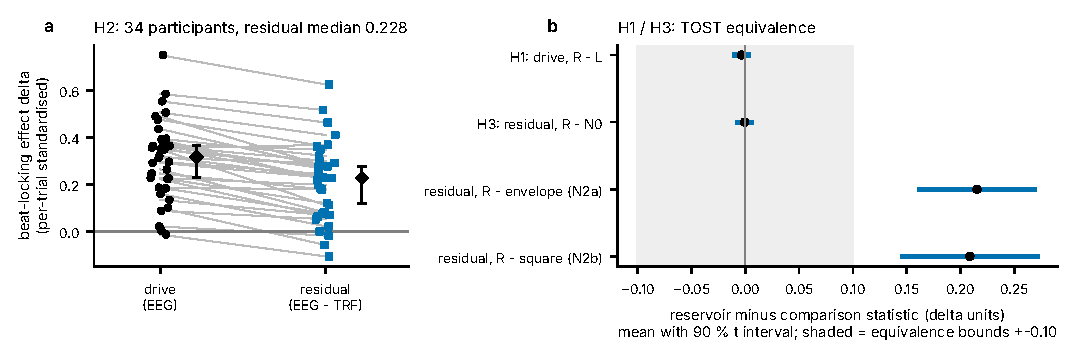
\includegraphics[width=\textwidth]{fig2_confirmatory.pdf}\caption{Confirmatory stage 2: H2 and H1/H3 equivalence.}\label{fig:conf}\end{figure*}
\begin{figure*}[!t]\centering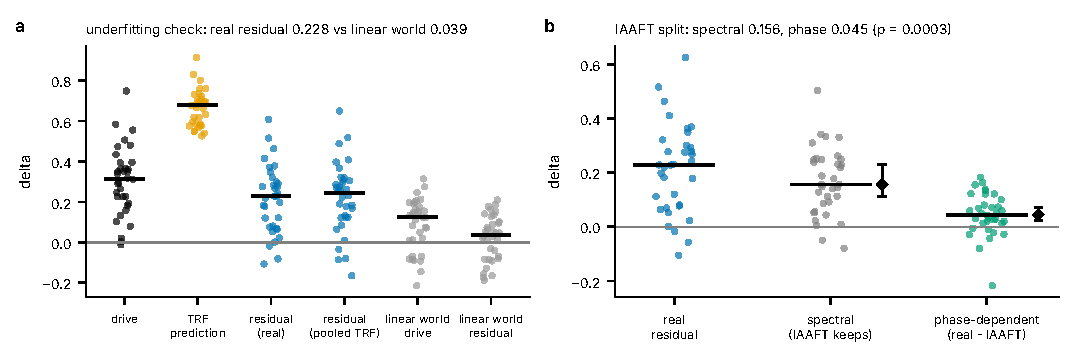
\includegraphics[width=\textwidth]{fig3_underfit_iaaft.pdf}\caption{Underfitting check and IAAFT decomposition (exploratory).}\label{fig:under}\end{figure*}
\begin{figure*}[!t]\centering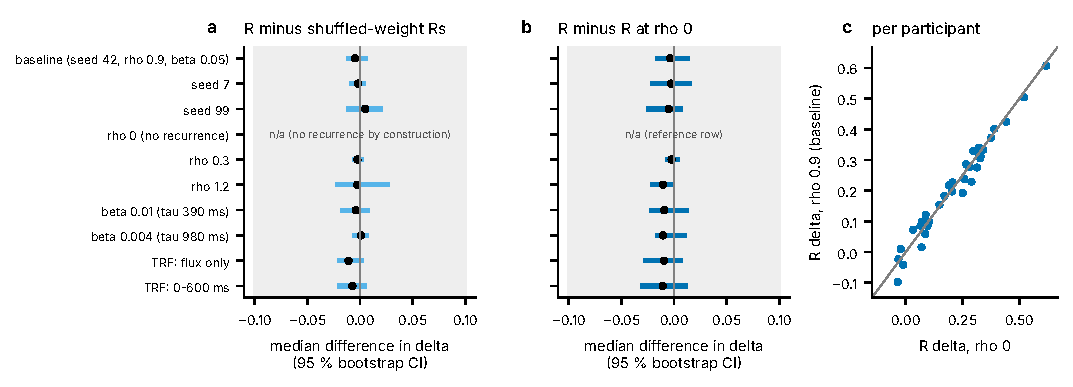
\includegraphics[width=\textwidth]{fig4_reservoir.pdf}\caption{Reservoir versus shuffled weights and versus no recurrence (exploratory).}\label{fig:res}\end{figure*}
\begin{figure*}[!t]\centering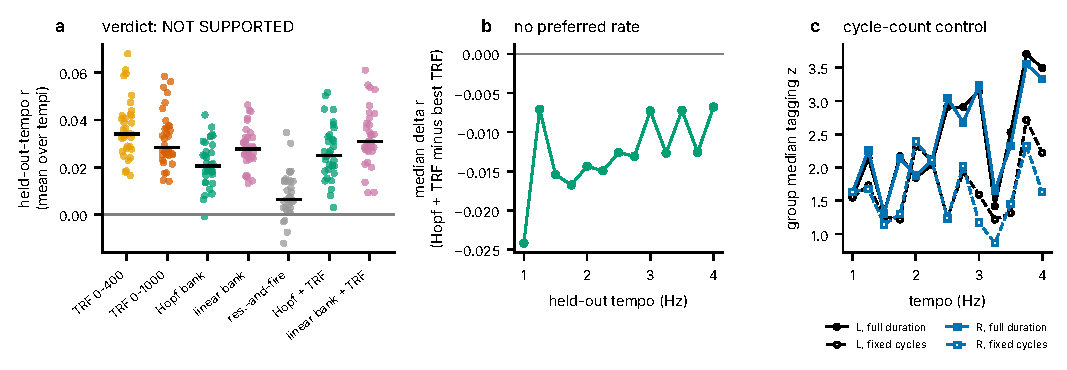
\includegraphics[width=\textwidth]{fig5_theory3.pdf}\caption{Oscillator encoding at held-out tempi and the cycle-count control (exploratory).}\label{fig:t3}\end{figure*}
\begin{figure*}[!t]\centering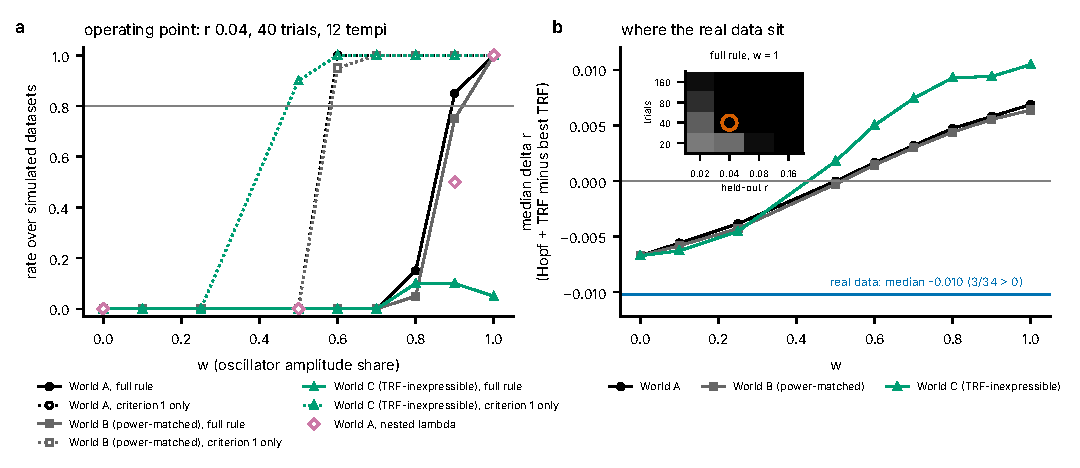
\includegraphics[width=\textwidth]{fig6_identifiability.pdf}\caption{Identifiability of an oscillator component (simulated).}\label{fig:ident}\end{figure*}
\begin{figure*}[!t]\centering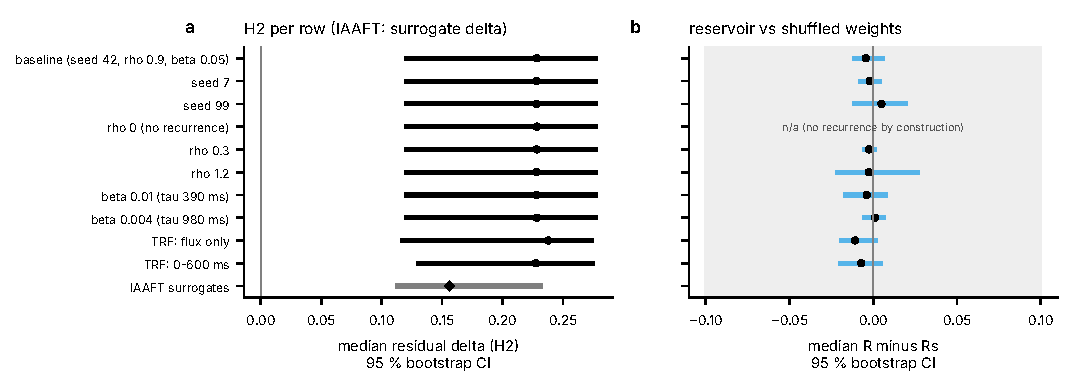
\includegraphics[width=\textwidth]{fig7_robustness.pdf}\caption{Robustness grid (exploratory).}\label{fig:rob}\end{figure*}

\bibliographystyle{IEEEtran}
\bibliography{references}
\end{document}
